\chapter{Current-State Analysis}

\section{Architecture Overview}
nopCommerce follows onion architecture, where all dependencies point inward toward the core. The solution is split into four main layers: \texttt{Nop.Core}, \texttt{Nop.Data}, \texttt{Nop.Services}, and the presentation layer (\texttt{Nop.Web} and \texttt{Nop.Web.Framework}).
\begin{figure}[h]
\centering
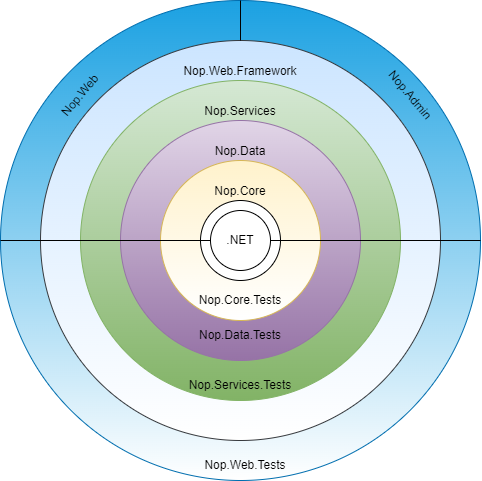
\includegraphics[width=0.68\textwidth]{images/nopCommerceArchitecture.png}
\caption{Current layered/onion architecture of nopCommerce.}
\label{fig:current-nopcommerce-architecture}
\end{figure}
Each layer has a specific role:
\begin{itemize}
\item \textbf{\texttt{Nop.Core}}: The innermost layer. Contains domain entities, caching, events, and helper classes shared across the whole solution. It has no dependencies on any other project. Key Scenario C entities live here: \texttt{Order}, \texttt{OrderItem}, \texttt{Product}, \texttt{ProductWarehouseInventory}, \texttt{StockQuantityHistory}, \texttt{Warehouse}, and \texttt{Shipment}.
\item \textbf{\texttt{Nop.Data}}: Separates data-access logic from business objects. nopCommerce uses a Linq2DB Code-First approach, with FluentMigrator for schema migrations and Fluent API for persistence mappings.
\item \textbf{\texttt{Nop.Services}}: The outermost layer of the Application Core. It holds business logic, validations, and calculations, and uses a repository pattern to expose features to layers above it. This is where order processing, inventory adjustment, shipping, and checkout logic live.
\item \textbf{\texttt{Nop.Web}} and \textbf{\texttt{Nop.Web.Framework}}: The presentation layer. \texttt{Nop.Web} contains controllers, models, views, and the storefront and admin area. \texttt{Nop.Web.Framework} is a shared class library with common presentation logic used by both the public site and the admin panel.
\item \textbf{Plugins}: Loaded as separate Visual Studio projects and extend nopCommerce for payments, shipping, authentication, search, and other integrations. They run inside the same runtime as the monolith.
\end{itemize}
\section{How a Purchase Works Today}
A customer order flows from the storefront controllers in \texttt{Nop.Web} down through \texttt{Nop.Services}. \texttt{OrderProcessingService} creates the order, adjusts inventory, persists state via repositories, and publishes internal events like \texttt{OrderPlacedEvent}. Shipment updates follow later through shipment services, which update order status and trigger notification events.
This works cleanly when nopCommerce owns the full picture. It breaks down when an external warehouse, POS, or carrier system owns part of the order's lifecycle and may be slow, unavailable, or return conflicting data.
The internal event system is also worth noting. It publishes events in-process to registered consumers and awaits each one. If a consumer fails, the error is logged and execution continues. There is no message broker and no standard durable integration retry, replay, or dead-letter mechanism. This is fine for cache invalidation or plugin reactions — it is not sufficient for reliable integration with external systems.
\section{What Already Works for Scenario C}
The current implementation already provides several Scenario C-relevant capabilities inside the monolith: web checkout and order creation, a local stock and warehouse model, shipment and tracking records, customer/admin order visibility, and plugin or scheduled-task extension points.

\subsection{Order Capture and Customer Visibility}
nopCommerce has mature order management: customer accounts, checkout, payment status, order history, shipment tracking, admin screens, and notification emails. This gives Scenario C a solid foundation. The order placement workflow is a natural seam where an integration event like "order accepted for fulfillment" can be emitted — currently it only fires in-process, but extending it with a durable outbox is straightforward without touching checkout itself.
\subsection{Inventory and Warehouse Model}
The platform already models stock quantity, reserved quantities, warehouse assignments, and stock history. This is directly useful for omnichannel stock visibility. The limitation is that nopCommerce treats this as local application state — it has no concept of whether a stock number came from the WMS ten seconds ago or ten hours ago, or whether a POS sale has already reduced it.
\subsection{Fulfillment and Shipping}
Shipment entities, tracking numbers, shipping plugins, pickup-in-store support, and customer notifications for shipping progress are all present. These support buy-online-fulfill-elsewhere flows. The gap is that shipment state is currently set by administrators or computed inside nopCommerce — there is no first-class integration status like "sent to WMS," "warehouse delayed," or "awaiting carrier confirmation."
\subsection{Plugins and Scheduled Tasks}
The architecture is modular, making it compatible with a variety of third-party services including ERPs, PIMs, and POS systems through its Web API plugin. Scheduled tasks can run background work — retries, synchronization, cleanup — and are protected against overlapping execution. These are useful extension points for Scenario C, though they lack the reliability structure needed for durable integration on their own.
\section{What Does Not Work for Scenario C}
\subsection{No Durable Integration Path}
The biggest gap is that there is no outbox, no integration message lifecycle, and no retry state. When an order is placed and the warehouse system is down, nopCommerce has no built-in guarantee that a fulfillment command was recorded, will be retried, or can be reconciled later. Logging an error is not a recovery path — operators need to know whether the order is waiting, failed, duplicated, or already accepted.
\subsection{No Freshness or Source Metadata on External State}
Stock, shipment, and fulfillment data can come from WMS, POS, ERP, or manual admin updates. The current model stores a value but does not record where it came from, when it was last confirmed, or whether it conflicts with another source. Stale data looks identical to fresh data to both customers and operators.
\subsection{Synchronous Plugin Calls Expose the Customer to External Failures}
When a plugin calls an external system during checkout or shipping-rate calculation, a slow or failed response degrades the customer experience directly. Scenario C requires the commerce core to stay useful when surrounding systems degrade — accepting safe work, signaling degraded status, and deferring unsafe steps — rather than failing visibly.
\subsection{No Standard Failure State or Reconciliation Model}
There is no common status model for integration messages: no "pending," "retrying," "failed," or "dead-lettered" states. There is no correlation between a placed order, the fulfillment command sent from it, and the acknowledgement (or conflict) that comes back. This makes recovery from partial failures opaque.
\subsection{Shared Database Must Stay Internal}
The nopCommerce database blends catalog, orders, customers, stock, shipments, configuration, and logs. This is fine for a monolith. It becomes a problem if external adapters start reading or writing it directly. Presentation logic in \texttt{Nop.Web} is isolated from the database — controllers only reference services, not repositories directly. The same discipline must apply at system boundaries: any fulfillment adapter, stock projection, or integration worker must communicate through APIs or events, not by coupling to nopCommerce tables.
\section{Useful Seams for Evolution}
The architecture provides clear attachment points without requiring a rewrite:
\begin{itemize}
\item \textbf{Order placement}: emit a durable integration message for fulfillment and ERP immediately after an order is accepted.
\item \textbf{Shipment updates}: receive warehouse and carrier progress and update nopCommerce shipment projections and customer-visible status.
\item \textbf{Inventory}: receive stock changes from WMS or POS and update a customer-facing availability view with freshness metadata.
\item \textbf{Scheduled tasks}: run outbox publishing, retry logic, timeout detection, and reconciliation outside the customer request path.
\item \textbf{Plugins and APIs}: connect to surrounding systems through explicit adapters, not direct database access.
\item \textbf{Admin visibility}: expose integration status, failures, and reconciliation actions to operators.
\end{itemize}
\section{What This Means for the Target Architecture}
nopCommerce should remain the owner of checkout, order management, customer visibility, catalog, and administration. Moving those out would create unnecessary scope.
The evolution targets three specific gaps instead:
\begin{itemize}
\item \textbf{Reliable propagation}: fulfillment and ERP commands must leave through a durable asynchronous path, not in-process events or direct plugin calls.
\item \textbf{Visible degradation}: when WMS, POS, ERP, or carriers are slow, unavailable, or contradictory, the system should expose an honest state — pending, delayed, degraded, or reconciliation required — rather than silently serving stale data.
\item \textbf{Recovery and reconciliation}: retries, idempotency, correlation identifiers, and operator-visible failure records should make it possible to recover without duplicating orders or hiding conflicts.
\end{itemize}
The current state is a strong starting point: it provides a real commerce base with genuine seams. The evolution adds reliability and cross-channel state visibility around the existing monolith rather than replacing it.
